\documentclass[a4paper,ngerman]{scrartcl}

\usepackage{amsmath}
\usepackage{amsfonts}
\usepackage{amssymb}
\usepackage[utf8]{inputenc}
\usepackage{graphicx}
\usepackage[ngerman]{babel}
\usepackage{hyperref}
\usepackage{float}
\usepackage{caption}
\usepackage{subcaption}
\usepackage{multirow}  %for tables
\usepackage{icomma} % Handle german comma as decimal point in numbers
\usepackage{units,siunitx} % Write units with correct spacing
\usepackage{upgreek} % provide non-italic greek letters
\usepackage{url}
%\usepackage{subfig}

% Formatting of table & figure captions
\captionsetup{font={sf,footnotesize},labelfont=bf,textfont=sl,skip=6pt}
\setlength{\abovecaptionskip}{6pt}
\setlength{\belowcaptionskip}{0pt}

\title{Black Lipid Membrane (BLM)}
\date{\today}
\author{Michel Rausch, Michael Eliachevitch}

\begin{document}

\maketitle
\tableofcontents
\newpage

\section{Einleitung}

In diesem Versuch werden Ionenkanäle in planaren Lipidmembranen untersucht. Hierbei wird der Wirkmechanismus des Antibiotikums Gramacidin A untersucht. In einer biologischen Zelle gelangen durch die entstandenen Kanäle Kationen durch die Zellmembran. Die Zelle stirbt aufgrund der Zerstörung ihres elektrochemischen Gradients [\ref{ref:mappe}].

Gramicidin beschreibt eine Gruppe Antibiotika. Dieses ist kommerziell unter Namen wie Angidin\textregistered , Mycolog\textregistered , Topsym\textregistered , Neospiron\textregistered  verfügbar. 


\section{Theoretische Grundlagen}

Die chemischen Grundlagen werden hier nicht genau behandelt. Gramicidin A1 besitzt die Summenformel $C_{99}H_{140}N_{20}O_{17}$. Es kann in der Natur von erdlebenden Bakterien beobachtet, aber auch synthetisch hergestellt werden. Mehrere Strukturen sind möglich, wobei Gramicidin A die häufigste ist. Gramicidin besitzt eine zyklische Struktur und damit einen anderen Wirkmechanismus. In diesem Experiment wird lediglich die Variante A verwendet.

\subsection{Wirkmechanismus}

Es existieren verschiedene Modelle, die Beschreiben, wie Gramicidin A (GA) in die Zellmembran integriert wird. Diese sind in Abbildung \ref{fig:wirkmechanismus} gezeigt. Auf die Einzelheiten wird nicht im Detail eingegangen.
\begin{itemize}
\item \textbf{A: Barrel Stave model} 
Hydrophobe, helixförmige Monomere bilden Poren in der Zellmembran.
\item \textbf{B: Toroidial Wormhole}  
Poremformation nahe phosphatidylethanolamine, oder phosphatidylserine Membranen. 
\item \textbf{C: Carpet model}  
Teppich-(engl. carpet-)ähnliche Anlagerung auf Membran.
\item \textbf{D} Detergent similar model
Bi- und Mizellen bilden Flächen auf der Membran. Durch deren Amphiphilie wird die Membran durchlässig.
\item \textbf{E} In-plane diffusion model
Verdünnung der Lipidschicht.
\end{itemize}

\begin{figure}
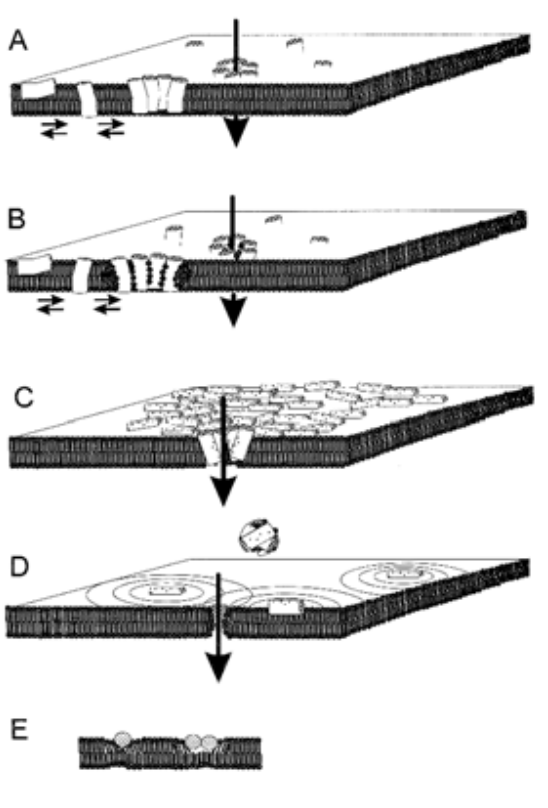
\includegraphics[width=0.5\textwidth]{wirkmechanismus.png}
\caption{Verschiedene Modelle zur Erklärung der Zerstörung einer Bakterienzelle mittels Peptid-Antibiotika [\ref{ref:mappe}]}
\label{fig:wirkmechanismus}
\end{figure}


\subsection{Ionentransport}

Eine Membran trennt zwei Bereiche einer wässrigen Lösung. Um sie zu überwinden, muss ein Ion eine Energie $E$ aufbringen. Die  Wahrscheinlichkeit k, eines Ions mit der Temperatur T, diese n einer Zeiteinheit zu überwinden ist der Ratenkoeffizient
\begin{equation} \label{eqn:rate}
k = k_0 e^{-\frac{E}{k_B T}},
\end{equation}
mit der Boltzmannkonstante $k_{B}$. Das Potential einer Membran lässt sich wie in Abbildung \ref{fig:potential-einfach} vorstellen. Die Ionen können in der Membran Bindungen eingehen, daher entstehen weitere Minima.

\begin{figure}
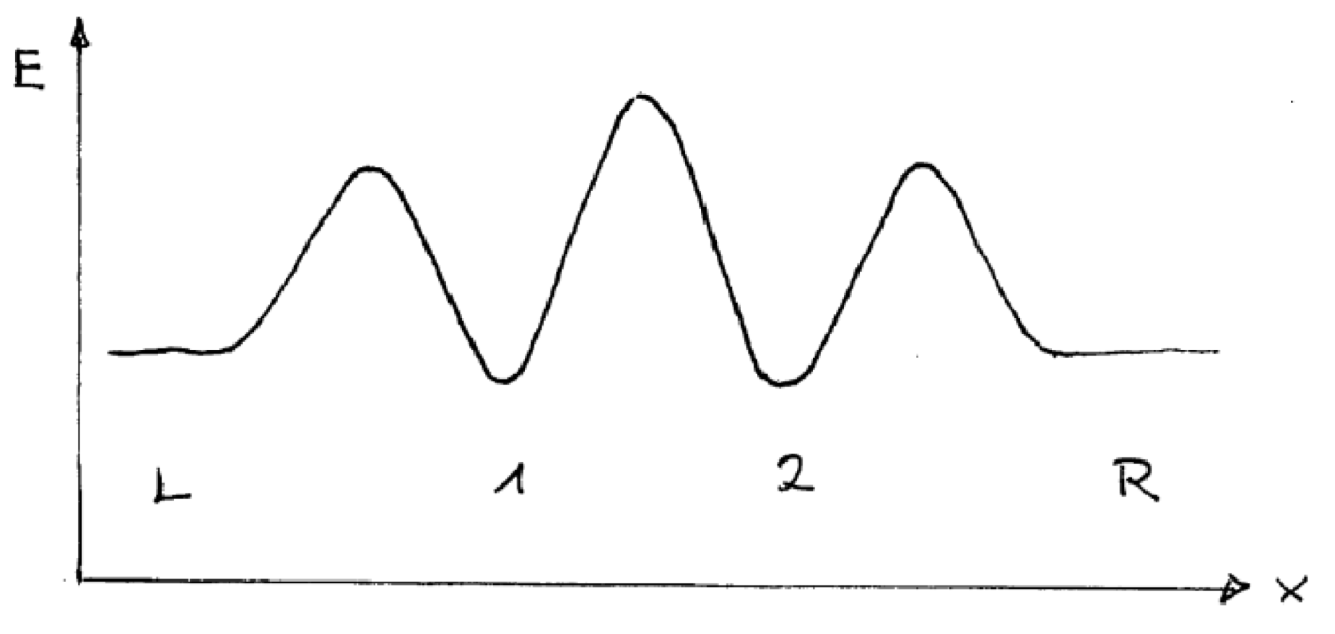
\includegraphics[width=0.6\textwidth]{potential-einfach.png}
\caption{Schema eines Potentials einer Pore [\ref{ref:mappe}]}
\label{fig:potential-einfach}
\end{figure}


Die Gleichung \ref{eqn:rate} wird auf den Fall des Experiments erweitert. Durch die angelegte Spannung $V_{m}$ wird das Potential asymmetrisch, wie in Abbildung \ref{fig:potential-asym} gezeigt.  Es wird die Quasistationaritätsnäherung verwendet. Die Leitfähigkeit eines einzelnen Kanals ist dann

\begin{equation}
\Gamma = \frac{k_A}{k_D} \cdot \frac{c}{k_A^{-1}+k^{-1}+k_D^{-1}} \cdot  \frac{q^2}{k_B T} .
\end{equation}

Mit der Ladung q der Ionen und den Ratenkoeffizienten $k_A$, $k_D$ und $k$ der Membran.
Hieraus ergeben sich die Zusammenhänge der makroskopisch Messbaren Größen

\begin{equation}
I_M = \lambda_M \cdot V_m
\end{equation}
und
\begin{equation}
\lambda_m = \Gamma \cdot N_p.
\end{equation}

Hierbei ist $I_M$ der gemessene Gesamtstrom an der Membran. $\lambda_M$ beschreibt die Leitfähigkeit der Membran.


\begin{figure}
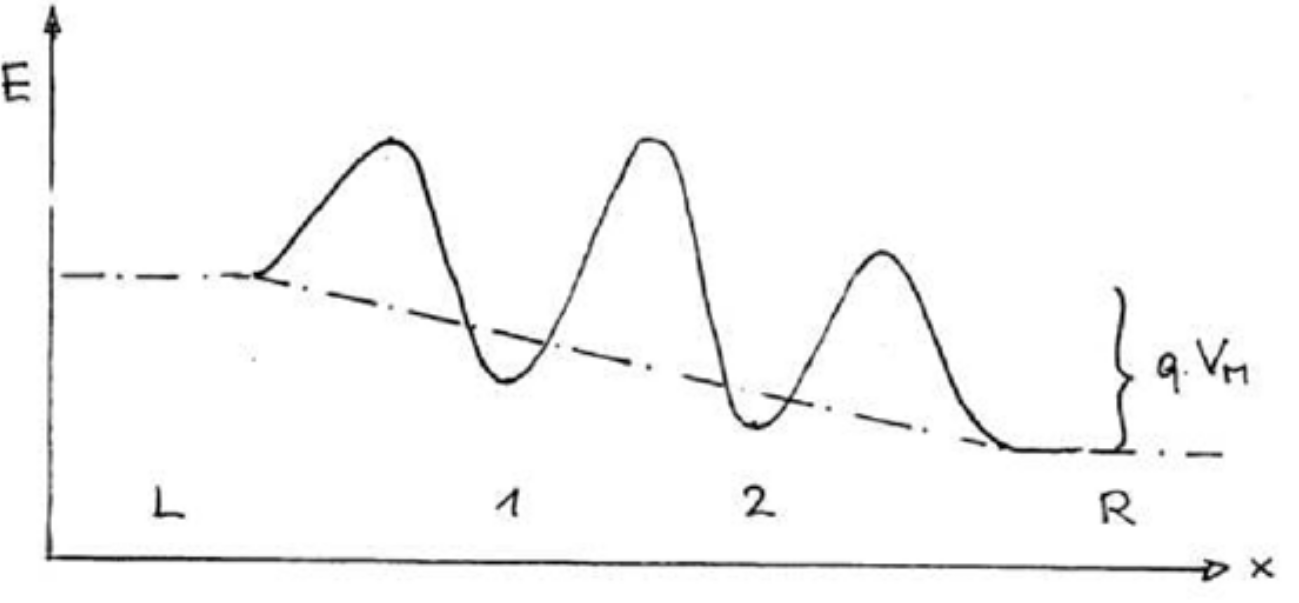
\includegraphics[width=0.6\textwidth]{potential-asym.png}
\caption{Schema eines Potentials einer Pore [\ref{ref:mappe}]}
\label{fig:potential-asym}
\end{figure}



\subsubsection{Einzelkanaltransport}




\subsubsection{Mehrkanaltransport}


\subsubsection{Autokorrelationsfunkion}


\subsubsection{Charakteristik einer Membran}






\section{Versuchsaufbau}

\begin{figure}[tb!]
  \centering
  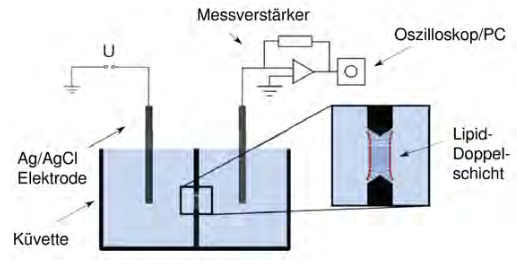
\includegraphics[width=0.9\textwidth]{abbildungen/blmaufbau.png}
  \caption{\textbf{Aufbau einer BLM ("`Black Lipid Membrane"').} \\Eine Küvette ist durch eine hydrophobe Trennwand zweigeteilt. Diese Trennwand hat ein kleines Loch in der Größenordnungen von Mikrometern, auf das die BLM "`aufgemalt"' ist. Die Küvette enthält eine Lösung und zwischen beiden Hälften kann durch Dioden eine Gleich- oder Wechselspannung angelegt werden. An einem Oszilloskop kann der Strom zwischen beiden Hälften beobachtet werden.}
  \label{fig:blmaufbau}
\end{figure}






\section{Aufgabenstellung und Versuchsdurchführung}

\subsection{Vorbereitung der Lipid-Doppelschicht}
\label{sec:bilayer-vorbereitung}

\subsection{Messung der Membran-Kapazität}
\label{sec:capacity}

\subsection{Messung einzelne Ionenkanäle}
\label{sec:singlechannels}

\subsection{Messung multipler Ionenkanäle}
\label{sec:multiplechannels}


\subsection{Noise-Analyse und Autokorrelationsfunktion}
\label{sec:noise-autocorr}

\subsection{Weitere Fragen}
\label{sec:weitere-fragen}















\section{Quellen}
\begin{enumerate}
\item Vorbereitungsmappe \label{ref:mappe}
\item pharmawiki.ch (16.11.2014) \label{ref:pharmawiki}
\end{enumerate}



\end{document}
